\section{Reinforcement Learning}

\begin{figure}[H]
    \centering
    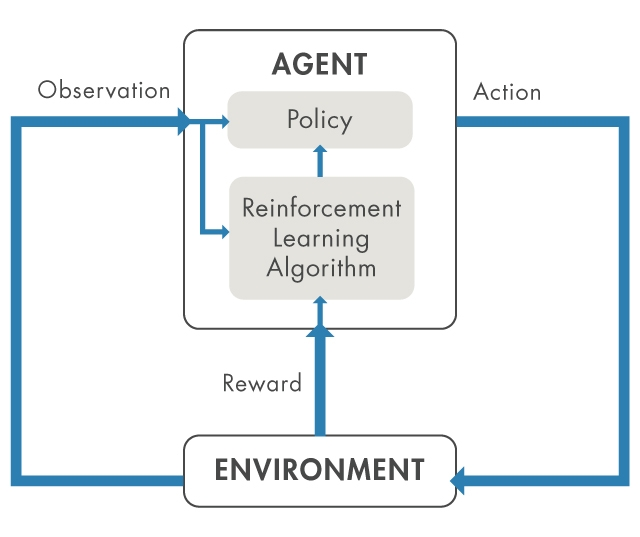
\includegraphics[scale=.4]{imm/reinforce.jpg}
    \caption{Diagramma riassuntivo del Reinforcement Learning}
\end{figure}

Normalmente, o almeno fin'ora, abbiamo visto che un errore implica un aggiustamento dell’ipotesi. L’errore è immaginato come una distanza tra comportamento presente e comportamento desiderato). Nel Reinforcement Learning, l’errore è rappresentato come premio o punizione per il comportamento; non c’è più la quantificazione di una distanza.\\ 

Al sistema viene associato un punteggio che dice se il sistema sta andando bene o male. E quindi di conseguenza i punti modificano le regole di comportamento del sistema.\\

Per esempio, all'interno di un gioco ci sono un ambiente, delle regole e delle interazioni che danno punti al nostro sistema. Normalmente nel Reinforcement Learning il sistema di punti è abbastanza generico perché non viene specificata la motivazione dietro al loro aumento o diminuzione. Non si sa esattamente come funziona l’ambiente, si sa solo interagire con esso, ovvero si possono compiere delle azioni nell’ambiente e farsi dire da quest’ultimo la nuova situazione dell’ambiente dopo l’azione.\\

Le decisioni di azione del sistema vengono prodotte da una politica interna di regole (policy) che si va via via a modificare tramite i punti ricevuti dall’ambiente stesso. L’algoritmo di Reinforcement Learning cambia la policy del sistema sulla base dei punti forniti dall’ambiente.

\subsection{Deep Learning}

Dalle reti neurali si passa a Deep Neural Net, ovvero reti neurali con più: strati (percettrone, backpropagation), algoritmi di discesa del gradiente, funzioni di attivazione, strumenti di regolazione comportando una maggior quantità di dati e una maggior potenza di calcolo.

\begin{figure}[H]
    \centering
    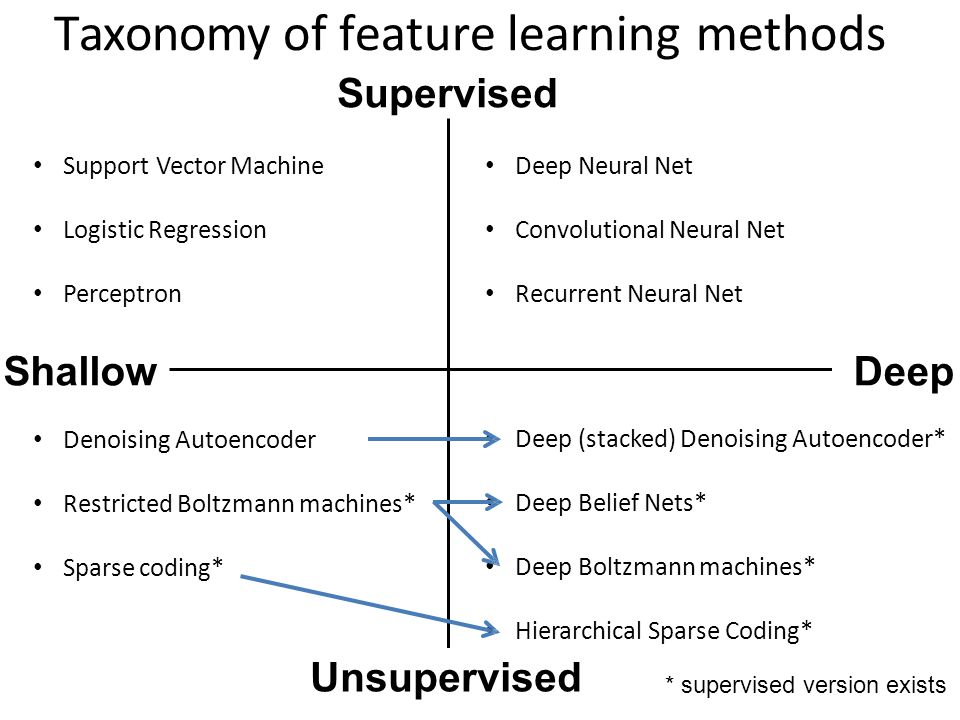
\includegraphics[scale=.4]{imm/deep-learn.jpg}
    \caption{Because some Deep Learning approaches are  considered to be Unsupervised -- it learns the features in the data  automatically (autoencoding)}
\end{figure}

La maggior parte degli algoritmi di Machine Learning non migliorano le proprie performance oltre una certa soglia di dati; mentre i nuovi metodi di deep learning riescono a sfruttare il continuo aumento dei dati, ottenendo un continuo miglioramento delle performance.\\

Nell’ambito dell’apprendimento su immagini, dal 2012 su è visto una sostanziale preferenza per i metodi di Deep Learning, a discapito di algoritmi più tradizionali.
Infatti gli algoritmi più tradizionali associavano alle immagini le feature corrispondenti in maniera manuale, mentre nel Deep Learning ciò avviene automaticamente tramite il sistema di apprendimento.\\

L’idea di un Multilayer Perceptron è quella di arricchire il comportamento delle reti aggiungendo layer e andando quindi in profondità. Ciò implica un aumento del numero di parametri (che potrebbe portare da overfitting) e un tempo di calcolo consistente. Sono quindi stati adottati alcuni rimedi per evitare questi effetti collaterali.\\

L’Autoencoder è una struttura (non profonda) shallow, non supervisionata che ha uno o più layer nascosti con un numero di unità nascoste minore del numero di feauture e che confronta i valori ottenuti in uscita con quelli forniti in ingresso. L’output è quindi in numero uguale al numero di feature in ingresso. \\
Questo modello produce quindi un errore (la distanza tra i vettori di input e output) che viene utilizzato per calcolare i pesi della rete.
Nell’hidden layer si ha una codifica (vettore di numeri in uno spazio a minor dimensioni) del dato di input.\\

Il Deep Learning è un set di algoritmi che imparano in layer, ovvero permettono al calcolatore di costruire una gerarchia di concetti compressi a partire da concetti più semplici.
Per esempio, per le immagini, si parte da un layer che contiene i pixel di input, passando a layer che man mano riconoscono linee, contorni, parti di oggetti fino all’identità degli oggetti.
Le feature vengono costruite automaticamente.

Struttura classica di apprendimento deep dedicato alle immagini
\begin{figure}[H]
    \centering
    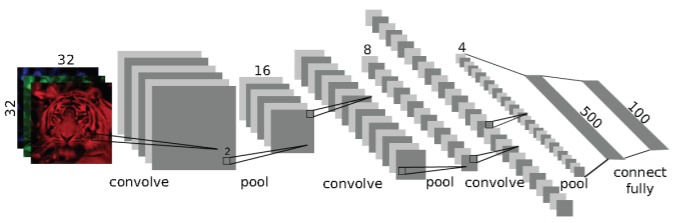
\includegraphics[scale=.8]{imm/imanges-deep.png}
\end{figure}

\textbf{\textit{Convoluzione}}\\

Al suo interno i neuroni sono connessi in un modo che evidenzia la struttura dei pixel nel campo visuale. Ciò è riprodotto nella connettività dei layer di certe reti. In origine un singolo neurone prendeva i segnali da tutti i pixel, ora invece un singolo neurone prende i segnali solo da una singola area di un’immagine. Un altro neurone prenderà i segnali da un’area spostata ma leggermente sovrapposta.\\

Ogni neurone quindi fa riferimento a una certa area-finestra dell’immagine e lo spostamento di questa finestra è ciò che viene definito convoluzione. La convoluzione rende evidente una struttura di adiacenza, non solo sui pixel di ingresso ma anche sui layer intermedi.\\

\textbf{\textit{Max pooling}}\\

Vede qual è il segnale più forte tra quelli ricevuti in ingresso e favorisce quello predominante. Il layer di pooling è formato da un gruppo di neuroni il cui segnale è trasformato nell’evidenza del più grande. Applicare l’operazione di pooling serve per ridurre l’immagine di input, riducendo quindi anche il numero di parametri.\\

Regolarizzare: combattere l’overfitting, sfumando lo spazio/ipotesi appreso.
Viene migliorata l’astrazione riducendo il numero di neuroni (dopo averli addestrati).